Správné řešení atomu vodíku je jedním z~velkých vítězství kvantové mechaniky. Podle klasické fyziky náboj, který se pohybuje se zrychlením (elektron obíhající vodíkové jádro -- proton), by měl vyzařovat elektromagnetické záření. To ve svém důsledku vede ke ztrátě energie a elektron by nakonec spadl na atomové jádro. Atom vodíku by tak byl nestabilní, s~dobou života řádově 1~ps. Ovšem to nepozorujeme. Proč jsou atomy, počínaje atomem vodíku stabilní, vysvětluje až kvantová mechanika.

\subsection{Úvod}
\label{kap:ObecnyUvod}

Řešit atom vodíku znamená nalézt řešení Schrödingerovy rovnice s~příslušným hamiltoniánem
\begin{equation}
\hat{H} = -\frac{\hbar^2}{2m_e}\Delta - \frac{1}{4\pi\epsilon_0}\frac{e^2}{r} \mbox{,}
\label{rov:Vodik1}
\end{equation}
kde předpokládáme, že elektron o~hmotnosti $m_e$ se pohybuje v~coulombickém poli nehybného jádra -- protonu. Kdybychom chtěli uvažovat i pohyb jádra, řešili bychom dvoučásticovou Schrödingerovu rovnici tak jako v~kapitole \ref{kap:dvecastice}. Příslušná Schrödingerova rovnici by šla separovat, zvlášť na relativní pohyb elektronu a protonu a zvlášť na pohyb celé soustavy. Rovnice, která by popisovala relativní pohyb, by měla tvar rovnice \eqref{rov:Vodik1}, kde hmotnost elektronu by byla nahrazena redukovanou hmotností $\mu$ soustavy jádro plus elektron. Při řešení také nebudeme uvažovat spin elektronu.

Vzhledem k~tomu, že coulombický potenciál v~rovnici \eqref{rov:Vodik1} jde k~nule pro $r \rightarrow \infty$, jsou nevázané stavy vodíku s~energií $E\geq0$ nekvantované a odpovídají spojitému spektru energií. Stavy s~energií $E<0$ jsou vázané a kvantované, protože pro ně platí podmínka $\psi(r) \rightarrow 0$ pro $r \rightarrow \infty$ vyplývající z~coulombického potenciálu.

Problém řešení atomu vodíku má kulovou symetrii, proto je výhodné pracovat ve sférických souřadnicích $(r, \theta, \phi)$. Z~hamiltoniánu \eqref{rov:Vodik1} vidíme, že coulombický potenciál závisí pouze na radiální souřadnici $r$, jde o~pohyb v~centrálním poli. Proto kvadrát momentu hybnosti a~$z$-ová složka momentu hybnosti komutují s~hamiltoniánem (viz kapitola \ref{kap:dvecastice}). Atom vodíku tak můžeme popsat vlnovou funkcí
\begin{equation}
\psi(r, \theta,\phi) = \psi_{nlm}(r, \theta,\phi) \mbox{,}
\label{rov:Vodik2}
\end{equation} 
kde vlnová funkce je charakterizována trojicí kvantových čísel $n,l,m$. Kvantová čísla $l$ a $m$ jsme poznali v~kapitole \ref{kap:momenthybnosti}. Kvantové číslo $n$ odpovídá kvantování v~radiálním směru a plyne z~coulombického potenciálu v~rovnici \eqref{rov:Vodik1}. Vzhledem k~tomu, že potenciál závisí pouze na $r$, bude energie vázaných stavů atomu vodíku záviset pouze na kvantovém čísle $n$
\begin{equation}
E = E_n \mbox{.}
\label{rov:Vodik3}
\end{equation}

\subsection{Spektrum energií}
\label{kap:SpektrumEnergii}

Začneme tím, že zapíšeme Schrödingerovu rovnici s~hamiltoniánem \eqref{rov:Vodik1} ve sférických souřadnicích
\begin{equation}
-\frac{\hbar^2}{2m_e} \left[ \frac{1}{r^2}\frac{\partial \psi}{\partial r} + \frac{1}{r^2 \sin \theta}\frac{\partial}{\partial \theta} \left( \sin \theta \frac{\partial \psi}{\partial \theta} \right) + \frac{1}{r^2 \sin^2 \theta}\frac{\partial^2 \psi}{\partial \phi^2}\right] - \frac{1}{4 \pi \epsilon_0}\frac{e^2}{r}\psi = E \psi \mbox{.}
\label{rov:Vodik4}
\end{equation}
Dále využijeme toho, že víme, že hamiltonián komutuje s~kvadrátem momentu hybnosti a $z$-ovu komponentou momentu hybnosti (viz \eqref{rov:2č-komutatorT}). Protože dva posledně jmenované operátory nezávisí na proměnné $r$ můžeme předpokládat separaci vlnové funkce \eqref{rov:Vodik2} ve tvaru
\begin{equation}
\psi(r, \theta, \phi) = R(r)Y_l^m(\theta, \phi) \mbox{,}
\label{rov:Vodik5}
\end{equation}
kde $R(r)$ je radiální část vlnové funkce a $Y_l^m(\theta, \phi)$ jsou sférické harmoniky, se kterými jsme se seznámili v~kapitole \ref{kap:momenthybnosti}. S~využitím separace proměnných a po malé úpravě (viz kapitola \ref{kap:dvecastice}) dostaneme radiální Schrödingerovu rovnici (viz vztah \eqref{rov:Radialni SCHR}) ve tvaru
\begin{equation}
-\frac{\hbar^2}{2m_e} \left[ \frac{1}{r^2}\frac{\mathrm{d}}{\mathrm{d} r} \left( r^2  \frac{\mathrm{d}}{\mathrm{d}r} \right) - \frac{l(l+1)}{r^2}\right]R - \frac{1}{4 \pi \epsilon_0}\frac{e^2}{r}R = E R \mbox{.}
\label{rov:Vodik6}
\end{equation}
Pro zájemce načrtneme způsob řešení této rovnice. Budeme postupovat tak, že nejprve zavedeme substituci $u=rR(r)$. Rovnice \eqref{rov:Vodik6} tak přejde na tvar
\begin{equation}
\frac{\mathrm{d}^2 u}{\mathrm{d}r^2}+ \frac{2m_e}{\hbar^2}\left[ \frac{e^2}{4 \pi \epsilon_0 r} - \frac{l(l+1)\hbar^2}{2 m_e r^2}\right]u = -\frac{2m_e E}{\hbar^2}u \mbox{.}
\label{rov:Vodik7}
\end{equation} 
Abychom rovnici dále zjednodušili zavedeme následující substituce
\begin{equation}
a = \left(\frac{2m_e}{\hbar^2} \right) \frac{e^2}{4\pi \epsilon_0}, \quad b=l(l+1), \quad \lambda^2 = \frac{2 m_e E}{\hbar^2} \mbox{,}
\label{rov:Vodik8}
\end{equation}
kde předpokládáme, že $E<0$, protože řešíme vázané stavy. Rovnice \eqref{rov:Vodik7} se dále zjednoduší na tvar
\begin{equation}
u^{\prime\prime} + \left( \frac{a}{r} - \frac{b}{r^2} \right) u = \lambda^2 u \mbox{,}
\label{rov:Vodik9}
\end{equation}
kde $u^{\prime\prime} = \mathrm{d}^2u/\mathrm{d}r^2$.

Nejprve vyřešíme rovnici \eqref{rov:Vodik9} pro případ, že $r \rightarrow \infty$, neboli asymptotické chování. Když je $r$ velké, přejde rovnice \eqref{rov:Vodik9} na tvar
\begin{equation}
u^{\prime\prime} \simeq \lambda^2 u \mbox{,}
\label{rov:Vodik10}
\end{equation}
kde symbolem $\simeq$ zdůrazňujeme, že řešení je přibližné a platí pouze v~limitě $r \rightarrow \infty$. Řešením této rovnice dostaneme
\begin{equation}
u\simeq e^{\pm \lambda r} \mbox{.}
\label{rov:Vodik11}
\end{equation}
Aby $u$ mohla vystupovat jako vlnová funkce, musí splňovat podmínku $u \rightarrow 0$ pro $r \rightarrow \infty$, protože jinak by nebylo možné funkci $u$ normalizovat (nebyla by kvadraticky integrovatelná). Proto fyzikálně smysluplným řešením je pouze
\begin{equation}
u\simeq e^{- \lambda r} \mbox{.}
\label{rov:Vodik12}
\end{equation}

\noindent Dále budeme předpokládat, že funkci $u$ můžeme zapsat jako
\begin{equation}
u = L(r) e^{-\lambda r} \mbox{,}
\label{rov:Vodik13}
\end{equation}
kde $L(r)$ je polynomická funkce v~$r$. Substitucí předpokladu \eqref{rov:Vodik13} do rovnice \eqref{rov:Vodik9} dostaneme (pozor, funkci $u$ musíme derivovat podle pravidla o~derivaci součinu funkcí)
\begin{equation}
L^{\prime\prime} -2\lambda L^{\prime} + \left( \frac{a}{r} - \frac{b}{r^2} \right) L =0 \mbox{.}
\label{rov:Vodik14}
\end{equation}
Řešení této rovnice budeme hledat ve tvaru
\begin{equation}
L(r) = \sum_n c_n r^n \mbox{,}
\label{rov:Vodik15}
\end{equation}
což po dosazení poskytne rovnici
\begin{equation}
\sum_n c_n \left\lbrace [n(n-1) - b]r^{n-2} - (2n\lambda - a)r^{n-1} \right\rbrace = 0 \mbox{.}
\label{rov:Vodik16} 
\end{equation}
Suma v~rovnici \eqref{rov:Vodik16} musí být rovna nule pro všechny hodnoty $r^n$. To bude splněno jen když bude platit rekurentní vztah mezi koeficienty
\begin{equation}
c_{n+1} = \left(\frac{2n\lambda - a}{n(n+1) - b}\right) c_n \mbox{.}
\label{rov:Vodik17}
\end{equation}
Aby tato řada vedla k~normalizované vlnové funkci $u$, musíme požadovat, aby řada přešla na polynom, tj. aby všechny koeficienty $c_n$ od dané hodnoty $n$ byly nulové. To se stane jen tehdy, když čitatel v~\eqref{rov:Vodik17} bude pro dané $n$ roven nule
\begin{equation}
2n\lambda = a \mbox{.}
\label{rov:Vodik18}
\end{equation}

Dosazením výsledku \eqref{rov:Vodik18} do substituce \eqref{rov:Vodik8} dostaneme pro hodnoty energie 
\begin{equation}
\boxed{E_n = - \frac{e^4 m_e}{32 \hbar^2 \pi^2 \epsilon_0^2} \frac{1}{n^2}, \quad n=1, 2, 3, \dots}
\label{rov:Vodik19}
\end{equation}
Znaménko mínus plyne z~toho, že řešíme vázané stavy, pro které platí $E<0$, což je v~souladu s~tím, že na ionizaci atomu ve vázaných stavech je potřeba dodat energii, například formou elektromagnetického záření. Zavedeme-li Bohrův atomový poloměr, který je dán vztahem
\begin{equation}
a_B = 4 \pi \epsilon_0 \frac{\hbar^2}{m_e e^2}
\label{rov:Vodik20}
\end{equation}
a dosadíme-li ho do rovnice \eqref{rov:Vodik19} dostaneme
\begin{equation}
E_n = - \frac{1}{4 \pi \epsilon_0}\frac{e^2}{2a_B}\frac{1}{n^2} \mbox{.}
\label{rov:Vodik21}
\end{equation}

Vidíme, že energie atomu vodíku závisí pouze na jediném kvantovém čísle $n$, které je spojeno s~radiálním pohybem. Kvantové číslo $n$ označujeme jako hlavní kvantové číslo. Máme-li zadanou hodnotu kvantového čísla $n$, nemůže být hodnota vedlejšího kvantového čísla $l$ libovolná, ale je určená relací
\begin{equation}
\boxed{l = 0, \dots, n-1 \mbox{.}}
\label{rov:Vodik22}
\end{equation}
Současně magnetické kvantové číslo $m$ nabývá hodnot
\begin{equation}
\boxed{m = -l, \dots, 0, \dots, +l \mbox{.}}
\label{rov:Vodik23}
\end{equation}
Série tří kvantových čísel parametrizuje daný kvantový stav. Povšimněme si skutečnosti, že pohyb ve 3D prostoru je popsán trojicí kvantových čísel, obdobně jako v~případě třírozměrné jámy v~kapitole \ref{kap:zakladniulohy}.

Energie základního stavu $E_1$ není degenerována, protože je popsána kvantovými čísly $n=1, l=m=0$, a její číselná hodnota se rovná $- 1 \,\mbox{Ry} = - 13,605 \,\mbox{eV}$. Energetická jednotka Rydberg (Ry) je definována jako
\begin{equation}
\mbox{Ry} = \frac{e^4 m_e}{32 \hbar^2 \pi^2 \epsilon_0^2}
\label{rov:Vodik24}
\end{equation}
a spolu s~Bohrovým atomovým poloměrem tvoří přirozené jednotky při popisu atomů.

Vyšší energetické stavy atomu vodíku $E_n, \,n=2,3,4, \dots$ jsou \textbf{degenerované}, protože jim přísluší více hodnot kvantových čísel $l$ a $m$. Pro každé $l$ máme celkem $2l+1$ hodnot $m$. Proto pro degeneraci hladiny $E_n$ dostaneme
\begin{equation}
g_n = \sum_{l=0}^{n-1}(2l+1) = n^2 \mbox{.}
\label{rov:Vodik25}
\end{equation}
Dále si můžeme všimnout toho, že energetické hladiny spektra vodíku nejsou od sebe vzdáleny ekvidistantně, jak tomu bylo v~případě harmonického oscilátoru, ale že vzdálenosti jednotlivých hladin se k~sobě blíží, když s~energií jdeme k~disociačnímu limitu, tj. $E_n=0$.

O~tom, že je spektrum vodíku složené z~diskrétních hladin svědčí i spektroskopická měření. Příčinou čárových atomových spekter je právě diskrétní charakter energetických hladin. Aby došlo k~přechodu elektronu mezi hladinami $f$ a $i$ musí dojít k~absorpci nebo emisi fotonu o~frekvenci dané rezonanční podmínku
\begin{equation}
\nu = \frac{|E_f-E_i|}{h} \mbox{.}
\label{rov:Vodik26}
\end{equation}
Podle toho jaká je hodnota kvantového čísla $n$, ze které pozorovaný přechod vychází, dělíme přechody do několika sérií: $n=1$ odpovídá Lymanově sérii v~UV oblasti, $n=2$ odpovídá Balmerově sérii ve viditelné oblasti a např. $n=3$ odpovídá Paschenově sérii v~IR oblasti.

\subsection{Vlnová funkce pro atom vodíku}
\label{kap:VlnovaFunkceVodik}

Celková vlnová funkce vázaných stavů atomu vodíku je součinem radiální části vlnové funkce a~sférických harmonik
\begin{equation}
\psi_{nlm}(r,\theta,\psi) = R_{nl}(r)Y_l^m(\theta, \phi)
\label{rov:Vodik30}
\end{equation}
a tvoří pro $n=1,2,3, \dots$, $l=0,\dots,n-1$ a$m=-l,\dots,+l$ úplný ortonormální systém funkcí, do kterého je možné rozvinout řešení nečasové Schrödingerovy rovnice pro vázané stavy.

Z~rekurentního vztahu \eqref{rov:Vodik17} můžeme dostat i vyjádření radiální části vlnové funkce $R_{nl}(\xi)$ ve tvaru
\begin{equation}
R_{nl}(\xi) = N_{nl} e^{-\xi/2}\xi^l L_{n+l}^{2l+1}(\xi) \mbox{,}
\label{rov:Vodik27}
\end{equation}
kde
\begin{equation}
\xi = \frac{2r}{n a_B}
\label{rov:Vodik28}
\end{equation}
a $L_{n+l}^{2l+1}(\xi)$ jsou tzv. \textbf{přidružené Laguerrovy polynomy}. Normovací koeficient je roven
\begin{equation}
N_{nl} = \left[ \left( \frac{2}{n a_B} \right)^3 \frac{(n-l-1)!}{2n[(n+l)!]^3}\right]^{1/2} \mbox{.}
\label{rov:Vodik29}
\end{equation}
Několik normovaných radiálních částí vlnových funkcí zde uvedeme
\begin{equation}
R_{10}(r) = \left( \frac{1}{a_B}\right) ^{3/2} 2 e^{-r/a_B} \mbox{,}
\end{equation}
\begin{equation}
R_{20}(r) = \left( \frac{1}{2a_B}\right) ^{3/2} \left(2-\frac{r}{a_B}\right) e^{-r/2a_B} \mbox{,}
\end{equation}
a
\begin{equation}
R_{21}(r) = \left( \frac{1}{2a_B}\right) ^{3/2} \frac{r}{a_B \sqrt{3}} e^{-r/2a_B} \mbox{.}
\end{equation}
Funkce jsou zobrazeny na obrázku~\ref{obr:RadialniFunkceVodik}.

Pravděpodobnost nalezení elektronu v~objemovém elementu $(r, r+ \mathrm{d}r)$, $(\theta,\theta+\mathrm{d}\theta)$ a $(\phi, \phi + \mathrm{d}\phi)$ je rovna
\begin{equation}
\mathrm{d}p (r, \theta, \phi) = |\psi_{nlm}(r, \theta, \phi)|^2 r^2 \mathrm{d}r \sin \theta \,\mathrm{d}\theta \mathrm{d}\phi \mbox{.}
\label{rov:Vodik31}
\end{equation} 
Integrací vztahu \eqref{rov:Vodik31} přes celý prostorový úhel získáme pravděpodobnost nalezení elektronu v~oblasti mezi $(r, r+ \mathrm{d}r)$
\begin{equation}
\mathrm{d}p (r) = |R_{nl}(r)|^2 r^2 \mathrm{d}r \mbox{,}
\label{rov:Vodik32}
\end{equation}
kde faktor $r^2 \sin \theta$ je Jakobián transformace z kartézských do sférických souřadnic. Výraz $P_{nl}(r)=|R_{nl}(r)|^2 r^2$ označujeme jako radiální hustotu pravděpodobnosti. Obdobně pro pravděpodobnost nalezení elektronu v~určitém prostorovém úhlu $(\theta,\theta+\mathrm{d}\theta)$ a $(\phi, \phi + \mathrm{d}\phi)$ získáme vztah
\begin{equation}
\mathrm{d}p (\theta, \phi) = |Y_{l}^m(\theta, \phi)|^2 \sin \theta \,\mathrm{d}\theta \mathrm{d}\phi \mbox{.}
\end{equation}
\begin{figure} [!ht]
\centering
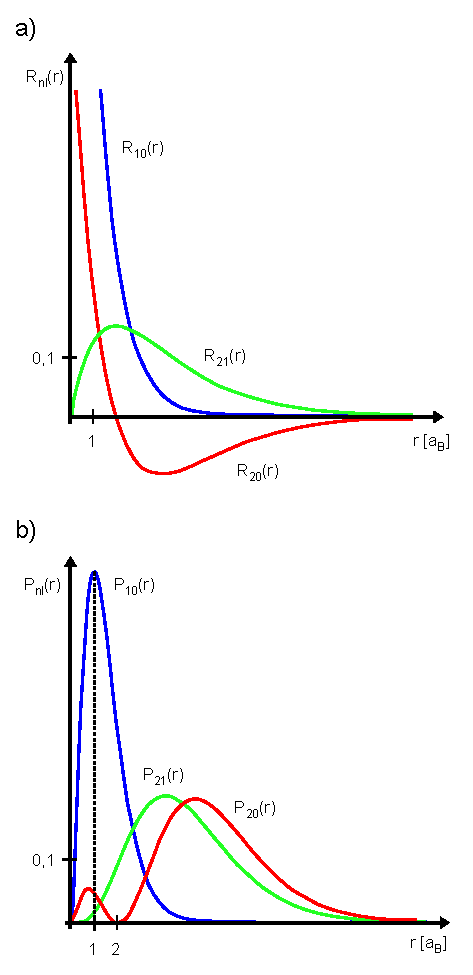
\includegraphics[scale=1]{vodik.pdf}
\caption[Radiální část vlnové funkce]{Na panelu a) jsou vyneseny 3 radiální části vlnové funkce $R_{10}$, $R_{20}$ a $R_{21}$ pro atom vodíku v~závislosti na souřadnici $r$, která je udaná v~jednotkách Bohrova poloměru $a_B$. Na panelu b) jsou vyneseny radiální hustoty pravděpodobnosti $P_{10}$, $P_{20}$ a $P_{21}$. Povšimněme si, že základní stav atomu vodíku $P_{10}$ má maximum hustoty ve vzdálenosti Bohrova poloměru $a_B$.}
\label{obr:RadialniFunkceVodik}
\end{figure}